\documentclass{report}
\usepackage[margin=1in, paperwidth=8.5in, paperheight=11in]{geometry}
%Math packages%
\usepackage{amsmath}
\usepackage{amssymb}
\usepackage{amsthm}
%Spacing%
\usepackage{setspace}
\onehalfspacing
%Lecture number%
\newcommand{\lectureNum}{13}
%Variables - Date and Course%
\newcommand{\curDate}{February 1, 2017}
\newcommand{\course}{MATH 239}
\newcommand{\instructor}{Luke Postle}
%Defining the example tag%
%\theoremstyle{definition}%
\newtheorem{ex}{Example}[section]
%Setting counter given the lecture number%
\setcounter{chapter}{\lectureNum{}}
%Package for drawing graphs%
\usepackage{tikz}
\usepackage{verbatim}
\usetikzlibrary{arrows}

\begin{document}
%Note title%
\begin{center}
\begin{Large}
\textsc{\course{} | Lecture \lectureNum{}}
\end{Large}
\end{center} 
\noindent \textit{Bartosz Antczak} \hfill
\textit{Instructor: \instructor{}} \hfill
\textit{\curDate{}}
\rule{\textwidth}{0.4pt}

% Actual Notes%
\subsubsection{Review of Last Lecture}
A \textbf{planar embedding} of a graph $G$ is a drawing of $G$ in the plane $\mathbb{R}^2$ such that the edges go between their ends and the interiors of distinct edges do not intersect. A graph is \textit{planar} if it has a planar embedding.
\section{Terminology with Planar Graphs}
\subsubsection{Definition 1 - Plane Graph}
A \textbf{plane graph} is a graph with a planar embedding.
\subsubsection{Terminology 1 - Face}
A \textit{face} $f$ of a plane graph $G$ is a connected region of $\mathbb{R}^2 - (E(G) \cup V(G))$
\begin{ex}
A graph with three faces, denoted as $f_1, f_2,$ and $f_3$
\end{ex}
\begin{center}
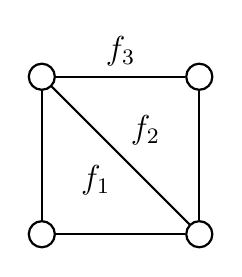
\begin{tikzpicture}[-,auto,node distance=2cm,
                    thick,main node/.style={circle,draw,font=\sffamily\small}]

  \node[main node] (1) {};
  \node[main node] (2) [right of=1] {};
  \node[main node] (3) [below of=1] {};
  \node[main node] (4) [right of=3] {};
  
  \path[every node/.style={font=\sffamily\large}]
    (1) edge node [above] {$f_3$} (2)
    	edge (3)
    	edge node [below left] {$f_1$}
    		node [above right] {$f_2$} (4)
    (4) edge (2)
    	edge (3);
\end{tikzpicture}
\end{center}
($f_3$, called the outer face, is unbounded).\\
The \textit{boundary} of a face is the set of all edges and vertices incident with it, where an edge (or similarly a vertex) is incident with a face if in its closure.\\
We say a face $f_1$ is \textit{incident} with a face $f_2$ if they are incident with a common edge (or adjacent).
\\ Let's consider a question:
\begin{center}
When is an edge incident with two faces?
\end{center}
From this question arises a proposition
\subsection{Proposition 1}
\begin{center}
\textit{An edge e is incident to exactly one face if and only if e is a bridge}
\end{center}
\subsubsection{Proof of Proposition}
\begin{itemize}
\item \textbf{($\implies$):} Suppose $e$ is incident to one face, but then in $G-e$, the ends of $e$ are in different components as they are separated by the face $f$. And hence, $e$ is a bridge.
\item \textbf{($\impliedby$):} Suppose $e$ is a bridge. Let $H_1, H_2$ be the two components of $G - e$ containing the ends of $e$ respectively. Then starting on one side of $e$, I can walk around the component $H_1$ and return to the other side of $e$. This implies that $e$ is only in one face, as desired.
\end{itemize}
\subsubsection{Definition 2 - Degree}
The \textbf{degree} of a face $f$ is the number of edges incident with $f$, where we count bridges twice.
\subsection{Handshaking Lemma for Faces}
Recall the handshaking lemma for the degrees of vertices on a graph. This lemma can be extended to faces as well:
$$\sum_{f} \mathrm{deg}(f) = 2\vert E(G) \vert$$
\subsubsection{Proof of Lemma}
Every edge in a cycle is incident to two different faces and so counted once in each of their degrees. Every bridge is in one face but is counted twice in its degree, QED.
\subsubsection{Getting Curious about Faces}
Let's ask another question:
\begin{center}
How many faces does a plane graph have?
\end{center}
The answer is constrained by the number of edges and vertices (let's denote them at $E$ and $V$ respectively, and let $F$ be the number of faces). For instance:
\begin{itemize}
\item A \underline{tree} has 1 face (where $E = V - 1$)
\item A \underline{cycle} has 2 faces (where $E = V$)
\item The graph from example 13.1.1 has 3 faces (where $E = V + 1$)
\end{itemize}
Observe that a little pattern starts to appear. This pattern is known as \textbf{Euler's formula}:
\begin{center}
\textit{If G is connected, then $V-E+F=2$}
\end{center}
How many edges does a forest have?
\subsubsection{Proposition 2}
\begin{center}
\textit{$E = V -$} (the number of components of $G$)
\end{center}
\subsubsection{Proof of Proposition 2}
Let $k$ be the number of components in $G$. Then $F$ is the disjoint union of trees, call them $T_1, \cdots, T_k$. But then $|E(T_i)| = |V(T_i)|-1$. If you sum $|E(G)| = |V(G)| - k$.
\subsubsection{Euler's General Formula}
Euler's formula can actually be expanded to not only apply to connected graphs:
\begin{center}
\textit{$V-E+F = 1\, +$} (number of components)
\end{center}
\subsubsection{Proof of Euler's General Formula}
We proceed by induction on $\vert E(G)\vert$. If $G$ is a forest, then $E=V - $ (number of components). So $V-E+F = V - (V - $ (number of components)) $ + \,1 = 1\, + $ (number of components), as desired.\\
So WMA, $G$ is not a forest. Thus there exists a cycle $C$, let $e \in E(C)$. Now $G-e$ is still a plane graph. But $|E(G-e)| = |E(G)| -1$, and $|V(G-e)| = |V(G)|$. Since $e$ is in a cycle, $e$ is not a bridge. So by proposition, $e$ is incident with two distinct faces, call them $f_1$ and $f_2$. So in $G-e$, all faces are the same, except $f_1$ and $f_2$ have merged into one face.\\
Thus, $|F(G-e)| = |F(G)| - 1$. Since $G-e$ has fewer edges than $G$, by induction: $|V(G-e)| - |E(G-e)| + |F(G-e)| = 1 +$ (\# of components of $G-e$). But $|V(G-e)| - |E(G-e)| + |F(G-e)| = |V(G)| - (|E(G)| - 1) + (|F(G)|-1) = |V(G)| - |E(G)| + |F(G)|$. Yet, the number of components of $G-e =$ (number of components of $G$ because $e$ is not a bridge). Thus, $V-E+F = 1+$ (number of components).
\subsubsection{So what good is Euler's Formula?}
It can determine whether a graph is planar or not. For example, recall $K_5$. If it were planar, then the number of faces would equal $E - V + 1 +$ (number of components) $= 10 - 5 + 1 + 1 = 7$.
Recall handshaking lemma for faces:
$$\sum_f \mathrm{deg}(f) = 2E = 20$$
But for all faces deg$(f) = 3$ (as long as not it's not $K_1$ or $K_2$). Then $\displaystyle \sum_f \mathrm{deg}(f) \geq 3F \geq 21$, a contradiction.
%END%
\end{document}